\chapter{Modélisation Mathématique}
\vspace{-1.5em}
\chaptertoc
\vspace{-2.5em}
\vspace{-0.3cm}
\section{Introduction}
Ce chapitre débute par une revue de littérature présentant les principales approches d'affectation des stands proposées dans les travaux antérieurs. Il introduit ensuite la modélisation du problème, en détaillant les contraintes identifiées, les algorithmes d'affectation retenus, ainsi que les hyperparamètres associés. Enfin, les métriques utilisées pour l’évaluation des performances.
\vspace{-0.5cm}
\section{Revue de littérature}
\label{sec:classical}
\vspace{-0.5em}
Dans cette section, nous présentons une revue des approches existantes permettant de résoudre le problème d’affectation des avions aux stands.

\vspace{-1em}
\subsection{Définition du problème}

L’\ac{SAP} joue un rôle essentiel dans la gestion aéroportuaire. Son objectif est d’attribuer à chaque avion une position au sol pour les opérations de débarquement, embarquement, maintenance et ravitaillement. Une allocation optimale améliore la fluidité des opérations, maximise l’utilisation des infrastructures et réduit les coûts, tout en garantissant la ponctualité des vols et le confort des passagers \cite{Das_2020}.
\vspace{-2.5em}
\begin{figure}[H]
	\centering
	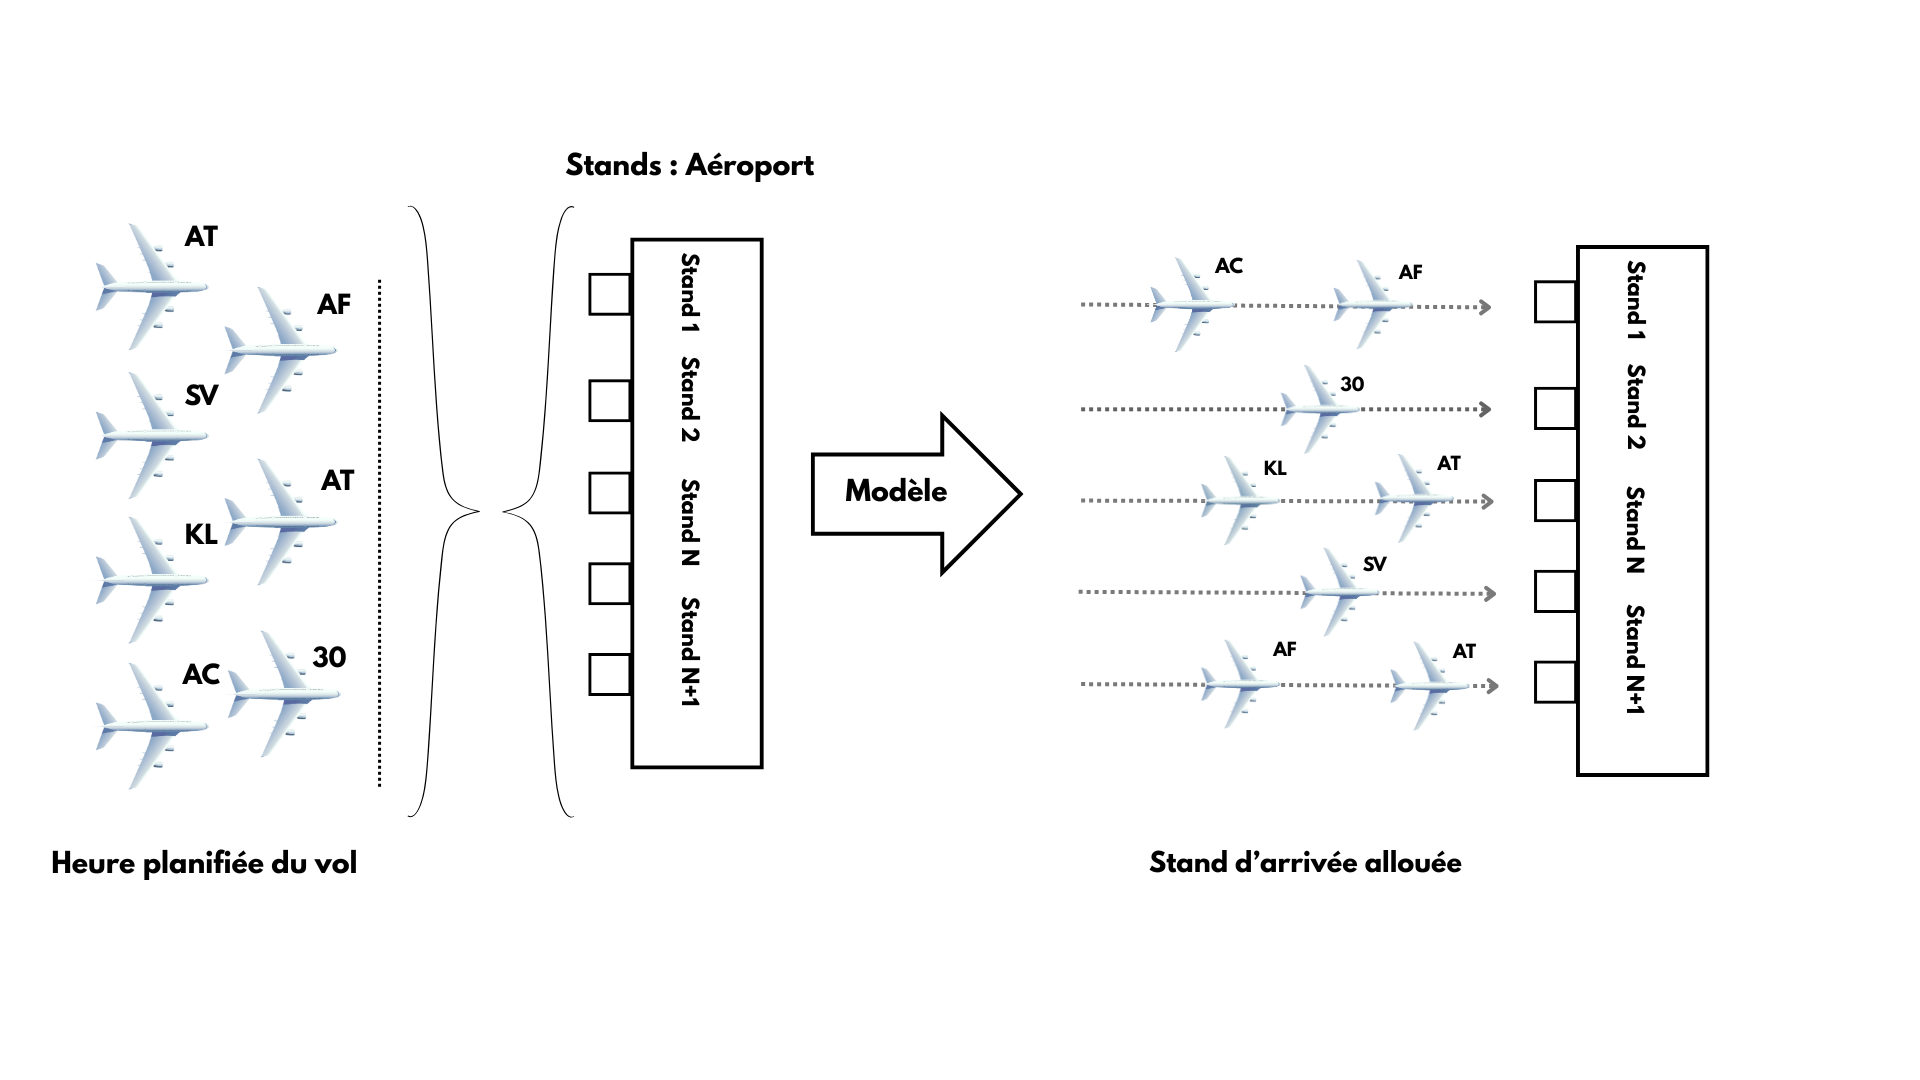
\includegraphics[width=0.7\linewidth]{assets/dataset/probleme.png}
	\caption{Définition du problème SAP}
	\label{fig:SAP}
\end{figure}
\vspace{-1.5em}
La figure \ref{fig:SAP} illustre le principe général de l’\ac{SAP}.  
Cependant, la résolution de l’\ac{SAP} représente un défi complexe en raison des multiples contraintes à prendre en compte : compatibilité avion/stand, contraintes temporelles, connexions entre vols et imprévus (tels que les retards). Ce problème, classé NP-difficile, devient rapidement ingérable par des méthodes exactes dans les grands aéroports, où des milliers de vols quotidiens — parfois plus de 300 par jour — doivent être répartis sur des dizaines de stands, générant un nombre astronomique de combinaisons possibles \cite{NilBusquetsTrias}.

Pour faire face à cette complexité, plusieurs approches d’optimisation ont été proposées et peuvent être regroupées en trois grandes catégories :
\begin{itemize}
	\item \textbf{Méthodes exactes}, qui garantissent une solution optimale sans violation des contraintes, mais sont limitées à des instances de petite taille et à des algorithmes spécialisés comme l’\textbf{algorithme hongrois} pour les problèmes d’affectation.
	\item \textbf{Heuristiques}, qui permettent d’obtenir des solutions approximatives rapidement.
	\item \textbf{Métaheuristiques}, qui explorent efficacement l’espace de recherche afin d’obtenir des résultats de haute qualité en un temps raisonnable.
\end{itemize}

Ces méthodes s’appliquent aussi bien à des contextes statiques, avec une planification préétablie, qu’à des contextes dynamiques nécessitant des ajustements en temps réel face aux imprévus et aux changements de dernière minute \cite{Cheng_2012}.

\subsection{Approches existantes}

Cette partie présente plusieurs approches d’optimisation qui ont été proposées.

\subsection*{Méthodes exactes}
\vspace{-0.5em}
Les méthodes exactes s’appuient sur une modélisation mathématique rigoureuse du problème d’\ac{SAP}, permettant de garantir l’optimalité des solutions pour des instances de taille raisonnable. Elles reposent principalement sur la \textbf{\ac{PL}}, \textbf{l'optimisation linéaire en nombres entiers} et les algorithmes de type \textbf{branch-and-bound} \cite{Bolat_2001,Li_2021}.
\vspace{-0.5em}
\subsubsection*{\small{\textcolor{blue}{Programmation Linéaire (PL/PLNE)}}}

\label{sec:LP}


L’\ac{SAP} est souvent modélisé comme un problème d’optimisation (linéaire ou mixte) visant à minimiser un coût (préférences, attente, déplacements). Il offre des résultats précis en temps raisonnable pour des cas moyens, mais peut exiger des ajustements manuels.

\textbf{Principe général :} La \ac{PL} optimise une fonction objectif linéaire sous des contraintes d’égalité et d’inégalité. Elle constitue la base de nombreux problèmes d’optimisation et se résout efficacement avec des algorithmes comme le simplexe. \textit{La solution optimale se trouve à un sommet de la région réalisable définie par les contraintes.}
\begin{algorithm}[H]
	\caption{Méthode du Simplexe pour la Programmation Linéaire}
	\label{alg:simplex}
	\begin{algorithmic}[1]
		\Require Coefficients de la fonction objectif $c$, matrice de contraintes $A$, bornes $b$
		\Ensure Solution optimale $x^*$ et valeur optimale $z^*$
		
		\State Convertir le problème en forme standard avec variables d'écart
		\State Initialiser une solution de base réalisable
		
		\Repeat
		\State Calculer les coûts réduits $c_j - c_B^T A_j$ pour toutes les variables non basiques
		\If{tous les coûts réduits $\geq 0$}
		\State \Return solution courante comme optimale
		\EndIf
		\State Sélectionner la variable entrante $x_k$ avec le coût réduit le plus négatif
		\State Calculer le vecteur direction $d = B^{-1} A_k$
		\If{$d \leq 0$}
		\State \Return le problème est non borné
		\EndIf
		\State Déterminer la variable sortante par le test du ratio minimal
		\State Mettre à jour la base et la solution
		\Until{convergence atteinte}
	\end{algorithmic}
\end{algorithm}
\vspace{-0.5em}
\textbf{Applications de recherche dans le SAP :}  
Pour dépasser les limites des modèles classiques, plusieurs auteurs ont introduit des extensions stochastiques afin de mieux gérer l’incertitude. Lim et al. \cite{Lim_2005} ont développé un modèle en deux étapes utilisant une distribution discrète pour représenter l’incertitude sur l’heure d’arrivée, basé sur la décomposition de Benders\footnote{La décomposition de Benders divise un problème en un problème maître et des sous-problèmes, facilitant sa résolution.}.

Dans une approche dynamique, Li et al. \cite{Li_2021} ont proposé un modèle multi-étapes basé sur des arbres de scénarios, intégrant décomposition hiérarchique et gestion du risque. Trias Busquets \cite{NilBusquetsTrias} a, de son côté, couplé \ac{PL} et \ac{GA} pour planifier l’affectation des stands.

\vspace{-0.5em}
\subsubsection*{\small{\textcolor{blue}{Méthodes Branch-and-Bound}}}


Les méthodes branch-and-bound explorent systématiquement l’espace des solutions en éliminant celles non optimales à l’aide de fonctions de bornes. Bien qu’elles garantissent l’optimalité, leur coût de calcul devient élevé pour les grandes instances.

\textbf{Principe général :}  
Partitionner systématiquement l’espace des solutions en sous-problèmes plus petits (ramification) et utiliser des bornes pour écarter ceux qui ne peuvent pas contenir la solution optimale, réduisant ainsi l’espace de recherche sans perdre la garantie d’optimalité.
\textbf{Applications de recherche dans le SAP :}  
Qin et al. \cite{Qin_2012} ont proposé une approche \textit{branch-and-price} exploitant la structure du problème via la génération de colonnes pour améliorer l’efficacité.


Guépet et al. \cite{Guepet_2016} ont développé un algorithme de \textit{branch-and-bound} enrichi par des coupes valides spécifiques à l’\ac{SAP}, intégrant également une phase de prétraitement permettant d’éliminer en amont les affectations incompatibles, réduisant ainsi l’espace de recherche.
\vspace{-0.5em}
\subsubsection*{\small{\textcolor{blue}{Algorithme Hongrois}}}
\label{sec:Hungarian}

\vspace{-0.5em}
L’algorithme hongrois est une méthode d’optimisation combinatoire spécialement conçue pour les problèmes d’affectation. Il constitue une approche spécialisée pour résoudre les problèmes de \ac{PL} carrée, dans lesquels le nombre d’agents et de tâches est égal.

\textbf{Principe général :}  
L’algorithme hongrois repose sur le fait que l’ajout ou le retrait d’une constante à une ligne ou une colonne de la matrice des coûts ne change pas l’affectation optimale.  
\textit{Il transforme progressivement la matrice par des réductions successives pour faire émerger un couplage parfait de coût minimal.}

\textbf{Applications de recherche dans le SAP :}  
Zhao et al. \cite{zhao2014algorithm} ont adapté l’algorithme hongrois, amélioré par Tomizawa, pour modéliser la planification du stationnement comme un problème d’affectation linéaire. Leur méthode minimise les distances de déplacement avec une complexité en \(O(N^3)\), garantissant une allocation optimale.

\vspace{-0.8em}
\subsection*{Algorithmes Heuristiques}

Les méthodes heuristiques offrent une alternative efficace aux approches exactes lorsque la taille du problème ou la complexité des contraintes rendent ces dernières impraticables. Elles visent à fournir des solutions de qualité satisfaisante, sans pour autant garantir leur optimalité.


\subsubsection*{\small{\textcolor{blue}{Algorithmes Gloutons}}}
\label{sec:Greedy}

\vspace{-0.5em}
Plusieurs travaux utilisent des heuristiques gloutonnes pour l’affectation des stands. Ces méthodes sont efficaces pour des instances moyennes, mais leur performance dépend de la structure du problème et de l’ordre de traitement des vols, sans possibilité de retour en arrière \cite{Ding_2004}.


\textbf{Principe général :} Choisir localement la meilleure option à chaque étape, sans revenir sur les décisions précédentes, en espérant atteindre un optimum global.
\begin{algorithm}[H]
	\caption{Hungarian Algorithm for Assignment Problem}
	\label{alg:hungarian}
	\begin{algorithmic}[1]
		\Require Cost matrix $C_{n \times n}$, where $c_{ij}$ is the cost of assigning task $j$ to agent $i$
		\Ensure Optimal assignment matrix $X_{n \times n}$ and minimum cost $z^*$
		
		\State Subtract the minimum value of each row and column from all elements of that row and column
		\Repeat
		\State Cover all zeros with a minimum number of horizontal or vertical lines
		\If{number of lines $<$ $n$}
		\State Find the smallest uncovered element $\theta$ and subtract it from all
		\State Add $\theta$ to elements at the intersection of covering lines
		\EndIf
		\Until{number of lines $=$ $n$}
		\State Extract optimal assignment from the final zero pattern
		\State \Return $X$, $z^* = \sum_{i,j} c_{ij} \cdot x_{ij}$
	\end{algorithmic}
\end{algorithm}

\vspace{-0.5em}
\textbf{Applications de recherche dans le SAP :}  
Ding et al. \cite{Ding_2004} ont proposé une heuristique gloutonne pour les cas de dépassement de capacités, visant à minimiser les vols non assignés et les distances.


\vspace{-0.7em}
\subsubsection*{\small{\textcolor{blue}{Recherche Tabou}}}


La recherche tabou est une métaheuristique guidant la recherche locale par une liste tabou des solutions récentes, évitant les cycles et favorisant l’exploration de nouvelles zones.

\textbf{Principe général :}  
Effectuer une recherche locale en mémorisant les déplacements récents pour éviter les retours en arrière et intensifier la recherche dans des régions prometteuses, avec des critères d’aspiration permettant de lever le statut tabou si nécessaire.

\textbf{Applications de recherche dans le SAP :}  
Ding et al. \cite{Ding_2004} ont combiné heuristiques gloutonnes et recherche tabou, introduisant le voisinage \textit{Interval Exchange Move}.  
Lim et al. \cite{Lim_2005} ont confirmé l’efficacité de la recherche tabou pour des cas complexes d’\ac{SAP}, grâce à sa capacité d’exploration.

\vspace{-0.5em}
\subsection*{Métaheuristiques et algorithmes évolutionnaires}

\vspace{-0.5em}
\subsubsection*{\small{\textcolor{blue}{Algorithmes Génétiques}}}
\label{sec:GA}
\vspace{-0.5em}

Les \ac{GA} s’inspirent de l’évolution naturelle pour optimiser des problèmes via sélection, croisement et mutation d’une population de solutions.

\textbf{Principe général :}  
Faire évoluer une population d’individus, favorisant la reproduction des plus adaptés, pour améliorer progressivement la qualité des solutions.

\textbf{Applications de recherche dans le SAP :}  
Gu et Chung \cite{Gu_1999} ont montré l’efficacité des AG pour la réaffectation dynamique des vols.  
Bolat \cite{Bolat_2001} les a utilisés pour minimiser le coût statique et les distances.  
Bagamanova et Mujica Mota \cite{Bagamanova_2018} ont combiné prédiction des retards et optimisation AG.  
Yang et Glover \cite{Yang_2007} ont proposé un AG hybride pour un planificateur à contraintes multi-niveaux.



\subsubsection*{\small{\textcolor{blue}{Recuit simulé}}}


Le \ac{SA} est une technique d’optimisation inspirée du processus de recuit en métallurgie. Elle accepte occasionnellement des solutions moins bonnes afin d’échapper aux optima locaux.

\textbf{Principe général :}  
Accepter les mouvements améliorants de façon déterministe, et les mouvements dégradants avec une probabilité décroissante à mesure que la "température" diminue, afin d’équilibrer exploration et exploitation tout au long de la recherche.  
 
\textbf{Applications de recherche dans le SAP :} Zhao et Duan \cite{Zhao_2021} ont démontré la supériorité des algorithmes génétiques simulés \ac{SA} par rapport aux modèles classiques dans des contextes aéroportuaires réels, en optimisant à la fois la minimisation des coûts et la maximisation de la satisfaction dans un cadre bi-objectifs.

\vspace{-0.8em}
\subsection*{Approches par Apprentissage par Renforcement}
\vspace{-0.5em}
L’apprentissage par renforcement a gagné en popularité pour résoudre le problème d’affectation aux stands (\ac{SAP}), en modélisant efficacement sa nature dynamique et stochastique.

\vspace{-0.5em}
\subsubsection*{\small{\textcolor{blue}{Processus de Décision de Markov Multi-Agents}}}
\vspace{-0.5em}

\textbf{Principe général :}  
Modéliser le \ac{SAP} comme un système multi-agents où les postes collaborent pour affecter les vols, apprenant des politiques optimales via leurs interactions avec l’environnement aéroportuaire dynamique.

\textbf{Applications de recherche dans le \ac{SAP}:}  
Aoun et El Afia \cite{Aoun_2018} ont proposé un cadre basé sur un PDM multi-agent temporel, capturant les incertitudes des vols et permettant une réaffectation collaborative respectant les contraintes opérationnelles.


\vspace{-0.5em}
\subsubsection*{\small{\textcolor{blue}{Apprentissage par Renforcement Profond}}}
\vspace{-0.5em}

\textbf{Principe général :}  
Associer réseaux neuronaux profonds et apprentissage par renforcement pour gérer de grands espaces d’états et apprendre des politiques complexes d’optimisation en temps réel de l’affectation des stands.

\textbf{Applications de recherche dans le SAP :}  
Li et al. \cite{Li_2025} ont proposé REGAPS, combinant un PDM adapté et l’architecture A3C pour optimiser en temps réel l’affectation des stands. Stein et al. \cite{Stein_2020} ont présenté un mécanisme d’apprentissage par renforcement assurant la stratégie pour l’allocation de ressources en ligne, applicable à l’affectation des stands.

\vspace{-1em}
\subsection*{Prise de Décision Multi-Critères}

Les méthodes de prise de décision multi-critères intègrent plusieurs objectifs et préférences des parties prenantes dans l’affectation des stands.

\textbf{Principe général :}  
Évaluer simultanément plusieurs critères en tenant compte des préférences et compromis entre objectifs conflictuels pour aboutir à des décisions équilibrées.

\textbf{Applications de recherche dans le SAP :}  
Skorupski et Żarów \cite{Skorupski_2014} ont proposé un modèle \ac{MCDM} prenant en compte les besoins spécifiques des acteurs aéroportuaires, offrant une allocation multi-critères personnalisée.

\vspace{-0.7em}
\subsection{Limites des approches existantes}

Les méthodes actuelles présentent plusieurs limites affectant leur efficacité en pratique :

\begin{itemize}
	\item \textbf{Dépendance au type de problème :} La \ac{PL} convient aux problèmes linéaires, tandis que les métaheuristiques sont mieux adaptées aux cas combinatoires.
	
	\item \textbf{Qualité vs temps :} Les méthodes exactes sont précises mais lentes, les heuristiques sont rapides mais souvent sous-optimales.
	
	\item \textbf{Scalabilité faible :} Les performances chutent face à de grands volumes de données.
	
	\item \textbf{Peu adaptées aux contextes dynamiques :} Les approches classiques ne gèrent pas bien les environnements évolutifs.
	
	\item \textbf{Gestion limitée des contraintes :} Certaines méthodes peinent à intégrer des contraintes complexes.
	
	\item \textbf{Sensibilité aux paramètres :} Les métaheuristiques nécessitent un réglage fin sans garantie d’optimalité globale.
\end{itemize}
\vspace{-1em}
\subsection{Justification du choix méthodologique}

Cette étude adopte une approche hybride combinant méthodes exactes, métaheuristiques et heuristiques, pour les raisons suivantes :

\begin{itemize}
	\item \textbf{Combinaison des forces :} Tirer parti de la rapidité et précision des méthodes exactes, tout en bénéficiant de la flexibilité et scalabilité des heuristiques et métaheuristiques.
	
	\item \textbf{Gestion de la complexité réelle :} Traiter des scénarios complexes et dynamiques avec des algorithmes robustes et adaptatifs.
	
	\item \textbf{Robustesse et flexibilité :} Adapter dynamiquement les structures de voisinage et particularités du problème, améliorant les performances.
	
	\item \textbf{Efficacité de la recherche :} Utiliser des algorithmes gloutons pour générer des populations initiales de qualité dans les \ac{GA}, accélérant la convergence.
\end{itemize}
\vspace{-1.2em}
\subsection{Synthèse et comparaison}
\vspace{-0.5em}
Cette section présente une synthèse complète des approches algorithmiques pour l’allocation des stands/gates (\ac{SAP}), résumée dans le tableau. La revue couvre 26 ans de recherche (1999-2025), montrant l’évolution des méthodes classiques vers l’apprentissage par renforcement, avec une récente focalisation sur des formulations multi-objectifs en temps réel.


\renewcommand{\arraystretch}{1.3}
\begin{table}[!htbp]
	\scriptsize
	\centering
	\label{tab:algorithmes}
	\caption{Synthèse des approches algorithmiques pour l’allocation des stands aéroportuaires}
	\begin{tabularx}{1.1\textwidth}{@{}p{3.3cm}p{3.2cm}p{3.7cm}p{3cm}p{2.3cm}@{}}
		\toprule
		Année/Auteur & Objectifs & Contraintes & Méthode & Mono/Bi-objectifs \\
		\midrule
		Gu et al.(1999) \cite{Gu_1999} & Réaffectation stand-avion & Contraintes de réaffectation & \textbf{Algorithme génétique} & Mono-objectif \\
		Bolat (2001) \cite{Bolat_2001} & Minimiser coût statique/distance & Coût ou distance & \textbf{Algorithme génétique} & Mono-objectif \\
		França et al. (2001) \cite{Franca_2001} & Allocation optimale des stands & Contraintes classiques & \textbf{Algorithme mémétique} & Mono-objectif \\
		Ding et al.(2004) \cite{Ding_2004} & Affectation sous contraintes & Contraintes d’affectation & \textbf{Glouton + Tabou} & Mono-objectif \\
		Lim et al. (2005) \cite{Lim_2005} & Planification avec fenêtres temporelles & Contraintes temporelles & \textbf{PL stochastique} & Mono-objectif \\
		Yang \& Glover (2007) \cite{Yang_2007} & Planification complexe & Contraintes multi-niveaux & \textbf{AG Hybride} & Mono-objectif \\
		Dorndorf et al.(2007) \cite{Dorndorf_2007} & Gestion des perturbations & Contraintes de robustesse & \textbf{Colonies de fourmis} & Mono-objectif \\
		Cheng et al. (2012) \cite{Cheng_2012} & Affectation des portes & Contraintes classiques & \textbf{Méthasheuristique} & Mono-objectif \\
		Qin et al. (2012) \cite{Qin_2012} & Affectation optimale des portes & Contraintes classiques & \textbf{Branch-and-Price} & Mono-objectif \\
		Skorupski \& Żarów (2014) \cite{Skorupski_2014} & Allocation multi-critères & Contraintes multi-critères & \textbf{\ac{MCDM}} & Bi-objectifs \\
		Guépet et al. (2016) \cite{Guepet_2016} & Optimisation combinée & Contraintes complexes & \textbf{Branch-and-Bound} & Mono-objectif \\
		Aoun \& El Afia (2018) \cite{Aoun_2018} & Réaffectation en temps réel & Contraintes opérationnelles & \textbf{MDP multi-agent} & Mono-objectif \\
		Bagamanova \& M.Mota (2018)\cite{Bagamanova_2018} & Minimiser retard via optimisation génétique & Contraintes de retard & \textbf{Algorithme génétique} & Mono-objectif \\
		Das et al.(2020) \cite{Das_2020} & Analyse multi-objectifs & Diverses contraintes & \textbf{Revue de littérature} & Multi-objectifs \\
		Stein et al. (2020) \cite{Stein_2020} & Allocation de ressources en ligne & Contraintes comportementales & \textbf{Apprentissage par renforcement contraint} & Mono-objectif \\
		Li et al. (2021) \cite{Li_2021} & Minimiser coût d’affectation & Contraintes d’affectation & \textbf{Programmation stochastique} & Mono-objectif \\
		Zhao \& Duan (2021) \cite{Zhao_2021} & Minimiser coût \& maximiser satisfaction & Contraintes stands & \textbf{Recuit simulé} & Bi-objectifs \\
		Trias Busquets (2024) \cite{NilBusquetsTrias} & Planification d’allocation des stands & Contraintes d’affectation & \textbf{Hybride PL + AG} & Mono-objectif \\
		Li et al. (2025) \cite{Li_2025} & Optimisation multi-objectifs temps réel & Contraintes disponibilité portes & \textbf{Apprentissage profond (DQN)} & Multi-objectifs \\
		\bottomrule
	\end{tabularx}

\end{table}
\vspace{-1em}
%-------------------------------------------------
\section{Modélisation mathématique}
%-------------------------------------------------
\vspace{-1em}
\subsection{Formulation du problème}

Le \ac{SAP} se modélise comme un programme
linéaire mixte en entiers dont l’objectif est d’affecter chaque vol à
un stand approprié, tout en respectant les contraintes et en minimisant les coûts.

Compte tenu de la nature combinatoire du problème, les méthodes exactes
deviennent rapidement impraticables à grande échelle. Nous adoptons donc
une approche hybride combinant des métaheuristiques \textbf{(Algorithmes
	génétiques, Tabu Search)} et des heuristiques pour explorer efficacement
l’espace de solutions.
%-------------------------------------------------
\subsection*{Variables de décision}
%-------------------------------------------------
\begin{itemize}
	\item $x_{is}\in\{0,1\}$ : vaut 1 si le vol $i$ est affecté au stand $s$, 0 sinon
	\item $y_{ijs}\in\{0,1\}$ : vaut 1 si le vol $j$ succède immédiatement au vol $i$ sur le stand $s$, 0 sinon
\end{itemize}

%-------------------------------------------------
\subsection{Paramètres}

%-------------------------------------------------
\subsubsection*{Paramètres liés aux vols}
\begin{itemize}
	\item $A_i$ : heure d’arrivée planifiée du vol $i$
	\item $D_i$ : heure de départ planifiée du vol $i$
	\item $a_i$ : taille de l’aéronef du vol $i$ (Small, Medium, Large, Super)
	\item $t_i$ : type du vol $i$ (Domestique, International)
	\item $schengen_i$ : 1 si le vol $i$ est Schengen, 0 sinon
\end{itemize}
\vspace{-0.8em}
\subsubsection*{Paramètres liés aux stands}
\begin{itemize}
	\item $A_s$ : accessibilité du stand $s$ (Contact, Remote)
	\item $s_s$ : taille maximale d’aéronef supportée par le stand $s$
	\item $schengen_s$ : 1 si le stand $s$ se trouve en zone Schengen, 0 sinon
\end{itemize}
\vspace{-0.5em}
%-------------------------------------------------
\subsection*{Notations complémentaires}
%-------------------------------------------------
\begin{itemize}
	\item $\mathcal{F}$ : ensemble de tous les vols
	\item $\mathcal{F}_{\text{int}}$, $\mathcal{F}_{\text{dom}}$ : vols internationaux / domestiques
	\item $\mathcal{S}$ : ensemble de tous les stands
	\item $\mathcal{S}_{\text{contact}}$, $\mathcal{S}_{\text{remote}}$ : stands contact / remote
	\item $\mathcal{T}_1$, $\mathcal{T}_2$, $\mathcal{T}_3$ : stands des terminaux 1, 2 et 3
	\item $\lambda_{\text{remote}}$ : pénalité d’utilisation d’un stand \textit{Remote} ($>1$)
	\item $\beta_1,\,\beta_2$ : poids de priorité pour les vols internationaux ($\beta_1>\beta_2>0$)
	\item $\gamma_1,\,\gamma_2$ : poids de priorité pour les vols domestiques   ($\gamma_1>\gamma_2>0$)
\end{itemize}
\vspace{-0.8em}
%-------------------------------------------------
\subsection{Formulation multi-objectifs}
%-------------------------------------------------

Le problème d’affectation de stands est naturellement multi-objectif ; nous
retenons la hiérarchie opérationnelle suivante :

\begin{tcolorbox}[colback=gray!10, colframe=gray,
	title={\textbf{Hiérarchie des objectifs opérationnels}}]
	\begin{enumerate}[label=\textbf{P\arabic*:}, leftmargin=2em]
		\item \textbf{	Optimisation de l’efficacité d’utilisation des stands et de l’expérience passager}
		\item \textbf{Optimiser les ressources et la compatibilité dimensionnelle}
	\end{enumerate}
\end{tcolorbox}


La formulation qui suit vise donc à équilibrer efficacité opérationnelle,
satisfaction passager et bonne utilisation des ressources au sein d’un
modèle unique.
\subsubsection{Objectif principal — Maximisation de l’utilisation des stands contact avec priorisation}
\label{sssec:primary_objective}

\begin{objective}[Affectation stratégique et efficace des stands]  
	
	
	L’objectif principal intègre l’efficacité opérationnelle et la satisfaction des passagers en :
	\begin{itemize}[leftmargin=1.7em]
		\item Maximisant l’utilisation des stands contact (équipés de passerelles),
		\item Réduisant le recours aux stands éloignés,
		\item Intégrant des préférences pondérées selon le type de vol, la localisation du terminal et l’accessibilité du stand.
	\end{itemize}
	
	Cela conduit à la formulation suivante :
	\begin{equation}
		\boxed{
			\max \quad Z_1 = \sum_{i \in \mathcal{F}} \sum_{s \in \mathcal{S}_{\text{contact}}} \omega(i,s) \cdot x_{is} - \lambda_{\text{remote}} \sum_{i \in \mathcal{F}} \sum_{s \in \mathcal{S}_{\text{remote}}} x_{is}
		}
		\label{eq:refactored_primary}
	\end{equation}
	où $\lambda_{\text{remote}} > 1$ est un coefficient de pénalisation, et $\omega(i,s)$ traduit la stratégie de priorisation.
\end{objective}

\noindent La fonction de pondération $\omega(i,s)$ est définie comme suit :
\begin{align*}
	\omega(i,s) = 
	\begin{cases}
		\beta_1 & \text{si } i \in \mathcal{F}_{\text{int}} \land s \in \mathcal{S}_{\text{contact}} \setminus \mathcal{T}_3 \\
		\beta_2 & \text{si } i \in \mathcal{F}_{\text{int}} \land s \in \mathcal{T}_3 \cap \mathcal{S}_{\text{contact}} \\
		\gamma_1 & \text{si } i \in \mathcal{F}_{\text{dom}} \land s \in \mathcal{T}_1 \cap \mathcal{S}_{\text{remote}} \\
		\gamma_2 & \text{si } i \in \mathcal{F}_{\text{dom}} \land s \in \mathcal{S}_{\text{remote}} \\
		0 & \text{sinon}
	\end{cases}
\end{align*}
avec $\beta_1 > \beta_2 > 0$ et $\gamma_1 > \gamma_2 > 0$ reflétant la hiérarchie des priorités.

\vspace{0.5em}
\noindent\textbf{Interprétation :}
\begin{itemize}[leftmargin=1.7em]
	\item Les vols internationaux ont la priorité maximale sur les stands contact hors Terminal 3.
	\item Les vols domestiques sont préférentiellement affectés aux stands éloignés du Terminal 1.
\end{itemize}

\subsubsection{Objectif secondaire — Optimisation des ressources dimensionnelles}
\label{sssec:secondary_objective}

\begin{objective}[Compatibilité stand-aéronef]
	
	L’objectif secondaire vise à minimiser l’écart entre la taille de l’aéronef et la capacité du stand afin d’éviter le sur-dimensionnement :
\vspace{-0.7em}
	\begin{equation}
		\boxed{
			\min \quad Z_2 = \sum_{i \in \mathcal{F}} \sum_{s \in \mathcal{S}} \phi(s_s, a_i) \cdot x_{is}
		}
		\label{eq:eq3}
	\end{equation}
	où $\phi(s_s, a_i) = \max(0, s_s - a_i)$ représente la pénalité liée à l’inadéquation des tailles.
\end{objective}

\noindent\textbf{Interprétation :}
\begin{itemize}[leftmargin=1.7em]
	\item Favorise l’affectation d’un aéronef à un stand de taille appropriée.
	\item Évite d’utiliser inutilement un grand stand pour un petit appareil.
\end{itemize}

\subsection{Scalarisation unifiée du problème multi-objectifs}

Pour fusionner les objectifs dans une seule fonction d’optimisation, nous utilisons une approche de scalarisation pondérée :
\vspace{-0.7em}
\begin{equation}
	\boxed{
		\min \quad \mathcal{J} = \sum_{i \in \mathcal{F}} \sum_{s \in \mathcal{S}} \mathcal{C}_{is} \cdot x_{is}
	}
\end{equation}

\noindent Le coût composite $\mathcal{C}_{is}$ intègre plusieurs composantes pondérées :

\begin{equation}
	\mathcal{C}_{is} = 
	\underbrace{\alpha_1 \cdot \mathcal{C}_1(a_i, A_s)}_{\text{Pénalité pour aéronef large sur stand éloigné}} +
	\underbrace{\alpha_2 \cdot \mathcal{C}_2(t_i, s, A_s)}_{\text{Alignement vol-terminal}} +
	\underbrace{\alpha_3 \cdot \mathcal{C}_3(s_s, a_i)}_{\text{Compatibilité de taille}}
\end{equation}
\subsubsection{Décomposition des composantes de coût}
\label{sssec:cost_breakdown}

Chaque composante de coût $\mathcal{C}_i$ correspond à un sous-objectif spécifique du modèle:

\paragraph{1. Pénalité pour gros porteurs sur stands éloignés (\ref{sssec:primary_objective})}  
\textit{Décourage l’affectation d’avions de grande taille ou super gros porteurs à des stands éloignés en raison de l’expérience passager dégradée et du coût opérationnel élevé.}
	\vspace{-0.7em}
\begin{equation}
	\mathcal{C}_1(a_i, A_s) = 
	\begin{cases}
		\kappa_{\text{large}} & \text{si } a_i \in \{\text{Large}, \text{Super}\} \land A_s = \text{Remote} \\
		0 & \text{sinon}
	\end{cases}
\end{equation}
avec $\kappa_{\text{large}} = 100$.

\paragraph{2. Optimisation vol-terminal (\ref{sssec:primary_objective})}  
\textit{Favorise l’affectation des vols domestiques aux terminaux préférés et pénalise les associations vol-terminal indésirables.}
	\vspace{-0.7em}
\begin{equation}
	\mathcal{C}_2(t_i, s, A_s) = 
	\begin{cases}
		-\rho_1 & \text{si } t_i = \text{Dom} \land s \in \mathcal{T}_1 \land A_s = \text{Remote} \\
		-\rho_2 & \text{si } t_i = \text{Dom} \land s \in \mathcal{T}_1 \land A_s = \text{Contact} \\
		-\rho_3 & \text{si } t_i = \text{Dom} \land s \in \mathcal{T}_3 \\
		+\rho_4 & \text{si } t_i = \text{Int} \land s \in \mathcal{T}_3 \\
		-\rho_5 & \text{si } t_i = \text{Int} \land s \notin \mathcal{T}_3 \land A_s = \text{Contact} \\
		0 & \text{sinon}
	\end{cases}
\end{equation}
avec $\rho_1 = 20$, $\rho_2 = 10$, $\rho_3 = 5$, $\rho_4 = 30$, et $\rho_5 = 25$.

\paragraph{3. Pénalité de sur-dimensionnement (\ref{sssec:secondary_objective})}  
\textit{Pénalise l’affectation d’un petit avion à un stand de grande taille afin d’éviter un gaspillage des ressources.}
	\vspace{-0.7em}
\begin{equation}
	\mathcal{C}_4(s_s, a_i) = 
	\begin{cases}
		\nu & \text{si } s_s > a_i \\
		0 & \text{sinon}
	\end{cases}
\end{equation}
		\vspace{-0.7em}     
avec $\nu = 5$.
		\vspace{-1em}     
\subsection{Contraintes}

Cette section présente les contraintes qui régissent l’affectation des vols aux stands dans un aéroport. Deux types de contraintes sont distingués : les contraintes dures et les contraintes souples.

\begin{tcolorbox}[colback=lightgraybox,colframe=gray,title={\textbf{Contraintes opérationnelles}}]
	\begin{enumerate}[label=\textbf{C\arabic*:}, leftmargin=2em]
		\item \textcolor{prioritycolor}{\textbf{Contraintes dures}} : doivent être strictement respectées afin de garantir la faisabilité de la solution. Elles assurent la conformité avec les règles opérationnelles et de sécurité.
		\item \textcolor{prioritycolor}{\textbf{Contraintes souples}} : peuvent être violées moyennant une pénalisation intégrée dans la fonction objectif. Ces contraintes visent à améliorer la qualité de service et l’efficacité de l’utilisation des ressources.
		Les contraintes souples sont prises en compte via les composantes de coût $\{\mathcal{C}_k\}_{k=1}^4$ de la section~\ref{sssec:cost_breakdown}.
	\end{enumerate}
\end{tcolorbox}

\subsubsection*{I– Contraintes dures}
\textit{Ces contraintes doivent impérativement être satisfaites pour garantir la validité de la solution.}
\begin{enumerate}
	
	\item \textbf{Affectation et occupation uniques par vol} :
	\vspace{-0.7em}
	\begin{equation}
		\sum_{s \in G} x_{is} = 1,\quad \forall i \in F \qquad \text{et} \qquad \sum_{i \in F} x_{is} \leq 1,\quad \forall s \in S
	\end{equation}
	Chaque vol doit être affecté à un seul stand, et chaque stand ne peut accueillir qu’un seul avion à un instant donné.
	
	\item \textbf{Compatibilité avion/stand} :
			\vspace{-0.7em}     
	\begin{equation}  
		a_i \cdot x_{is}  \leq s_s , \quad \forall i \in F,\; s \in S
	\end{equation}
	Un avion ne peut être affecté qu’à un stand compatible avec sa taille.
	
	\item \textbf{Incompatibilité physique entre certains stands} :
	\vspace{-0.7em}
	\begin{equation}
		\sum_{i \in F} x_{is} + \sum_{j \in F} x_{js'} \leq 1, \quad \forall (s, s') \in S
	\end{equation}
	Certains stands adjacents ne peuvent pas être utilisés simultanément (exemple : $J9 = B9 + B10$).
	
	\item \textbf{Non chevauchement temporel} :
			\vspace{-0.7em}     
	\begin{equation}
		x_{is} + x_{js} \leq 1, \quad \text{si } [A_i, D_i] \cap [A_j, D_j] \neq \emptyset
	\end{equation}
	Deux vols ne peuvent occuper le même stand au même moment.
	
	\item \textbf{Cohérence des successions sur un même stand} :
	\vspace{-0.7em}
	\begin{equation}
		\sum_{j \in F} y_{ijs} \leq x_{is}, \quad 
		\sum_{i \in F} y_{ijs} \leq x_{js}, \quad 
		\forall i, j \in F,\; s \in S
	\end{equation}
	Un vol $j$ peut succéder à un vol $i$ sur le même stand $s$ seulement si les deux y sont affectés.
	
	\item \textbf{Cohérence de la zone Schengen} :
\vspace{-0.7em}

\begin{equation}
	x_{is} \leq \mathds{1}_{schengen_i = schengen_s}
	, \quad \forall i \in F,\, s \in S
\end{equation}

	Un vol Schengen doit être affecté à un stand situé dans la même zone (Schengen ou non).
	
\end{enumerate}

%--------------------------------------------------
\vspace{-1.7em}
\section{Algorithmes utilisés}
\vspace{-0.5em}
Dans cette section, nous présentons une analyse complète des approches algorithmiques utilisées dans ce projet, incluant à la fois des techniques d’\textbf{optimisation classique} et des approches \textbf{hybrides modernes}. Le choix des algorithmes est motivé par la nécessité de résoudre des problèmes complexes nécessitant des solutions robustes, efficaces et adaptables. Notre approche combine plusieurs paradigmes algorithmiques pour tirer parti de leurs forces complémentaires.

Comme détaillé dans la revue de littérature (section~\ref{sec:classical}), des algorithmes classiques tels que \textbf{la Programmation Linéaire~\ref{sec:LP}, l’algorithme hongrois~\ref{sec:Hungarian}, l’algorithme glouton~\ref{sec:Greedy}, et l’algorithme génétique~\ref{sec:GA}} offrent des bases solides en matière d’optimisation. En s’appuyant sur ces approches, cette section met l’accent sur les \textbf{approches hybrides} combinant les forces de différents paradigmes pour améliorer la performance et la robustesse.

Les algorithmes hybrides présentés ici représentent des combinaisons innovantes conçues pour exploiter les effets synergiques de différentes stratégies d’optimisation. Nous nous concentrons sur deux approches principales :

\begin{itemize}
	\item Algorithme hybride génétique glouton  : \textbf{GGA}
	\item Algorithme hybride recuit simulé et recherche tabou : \textbf{TSSA}
\end{itemize}
\vspace{-1.7em}
\subsection*{Algorithme Génétique Glouton (GGA)}
\vspace{-0.5em}
Cette section décrit l’algorithme génétique glouton hybride (GGA), qui combine la génération rapide de solutions par des heuristiques gloutonnes avec la capacité d’exploration globale des algorithmes génétiques.
\vspace{-0.9em}     
\begin{figure}[H]
	\centering
	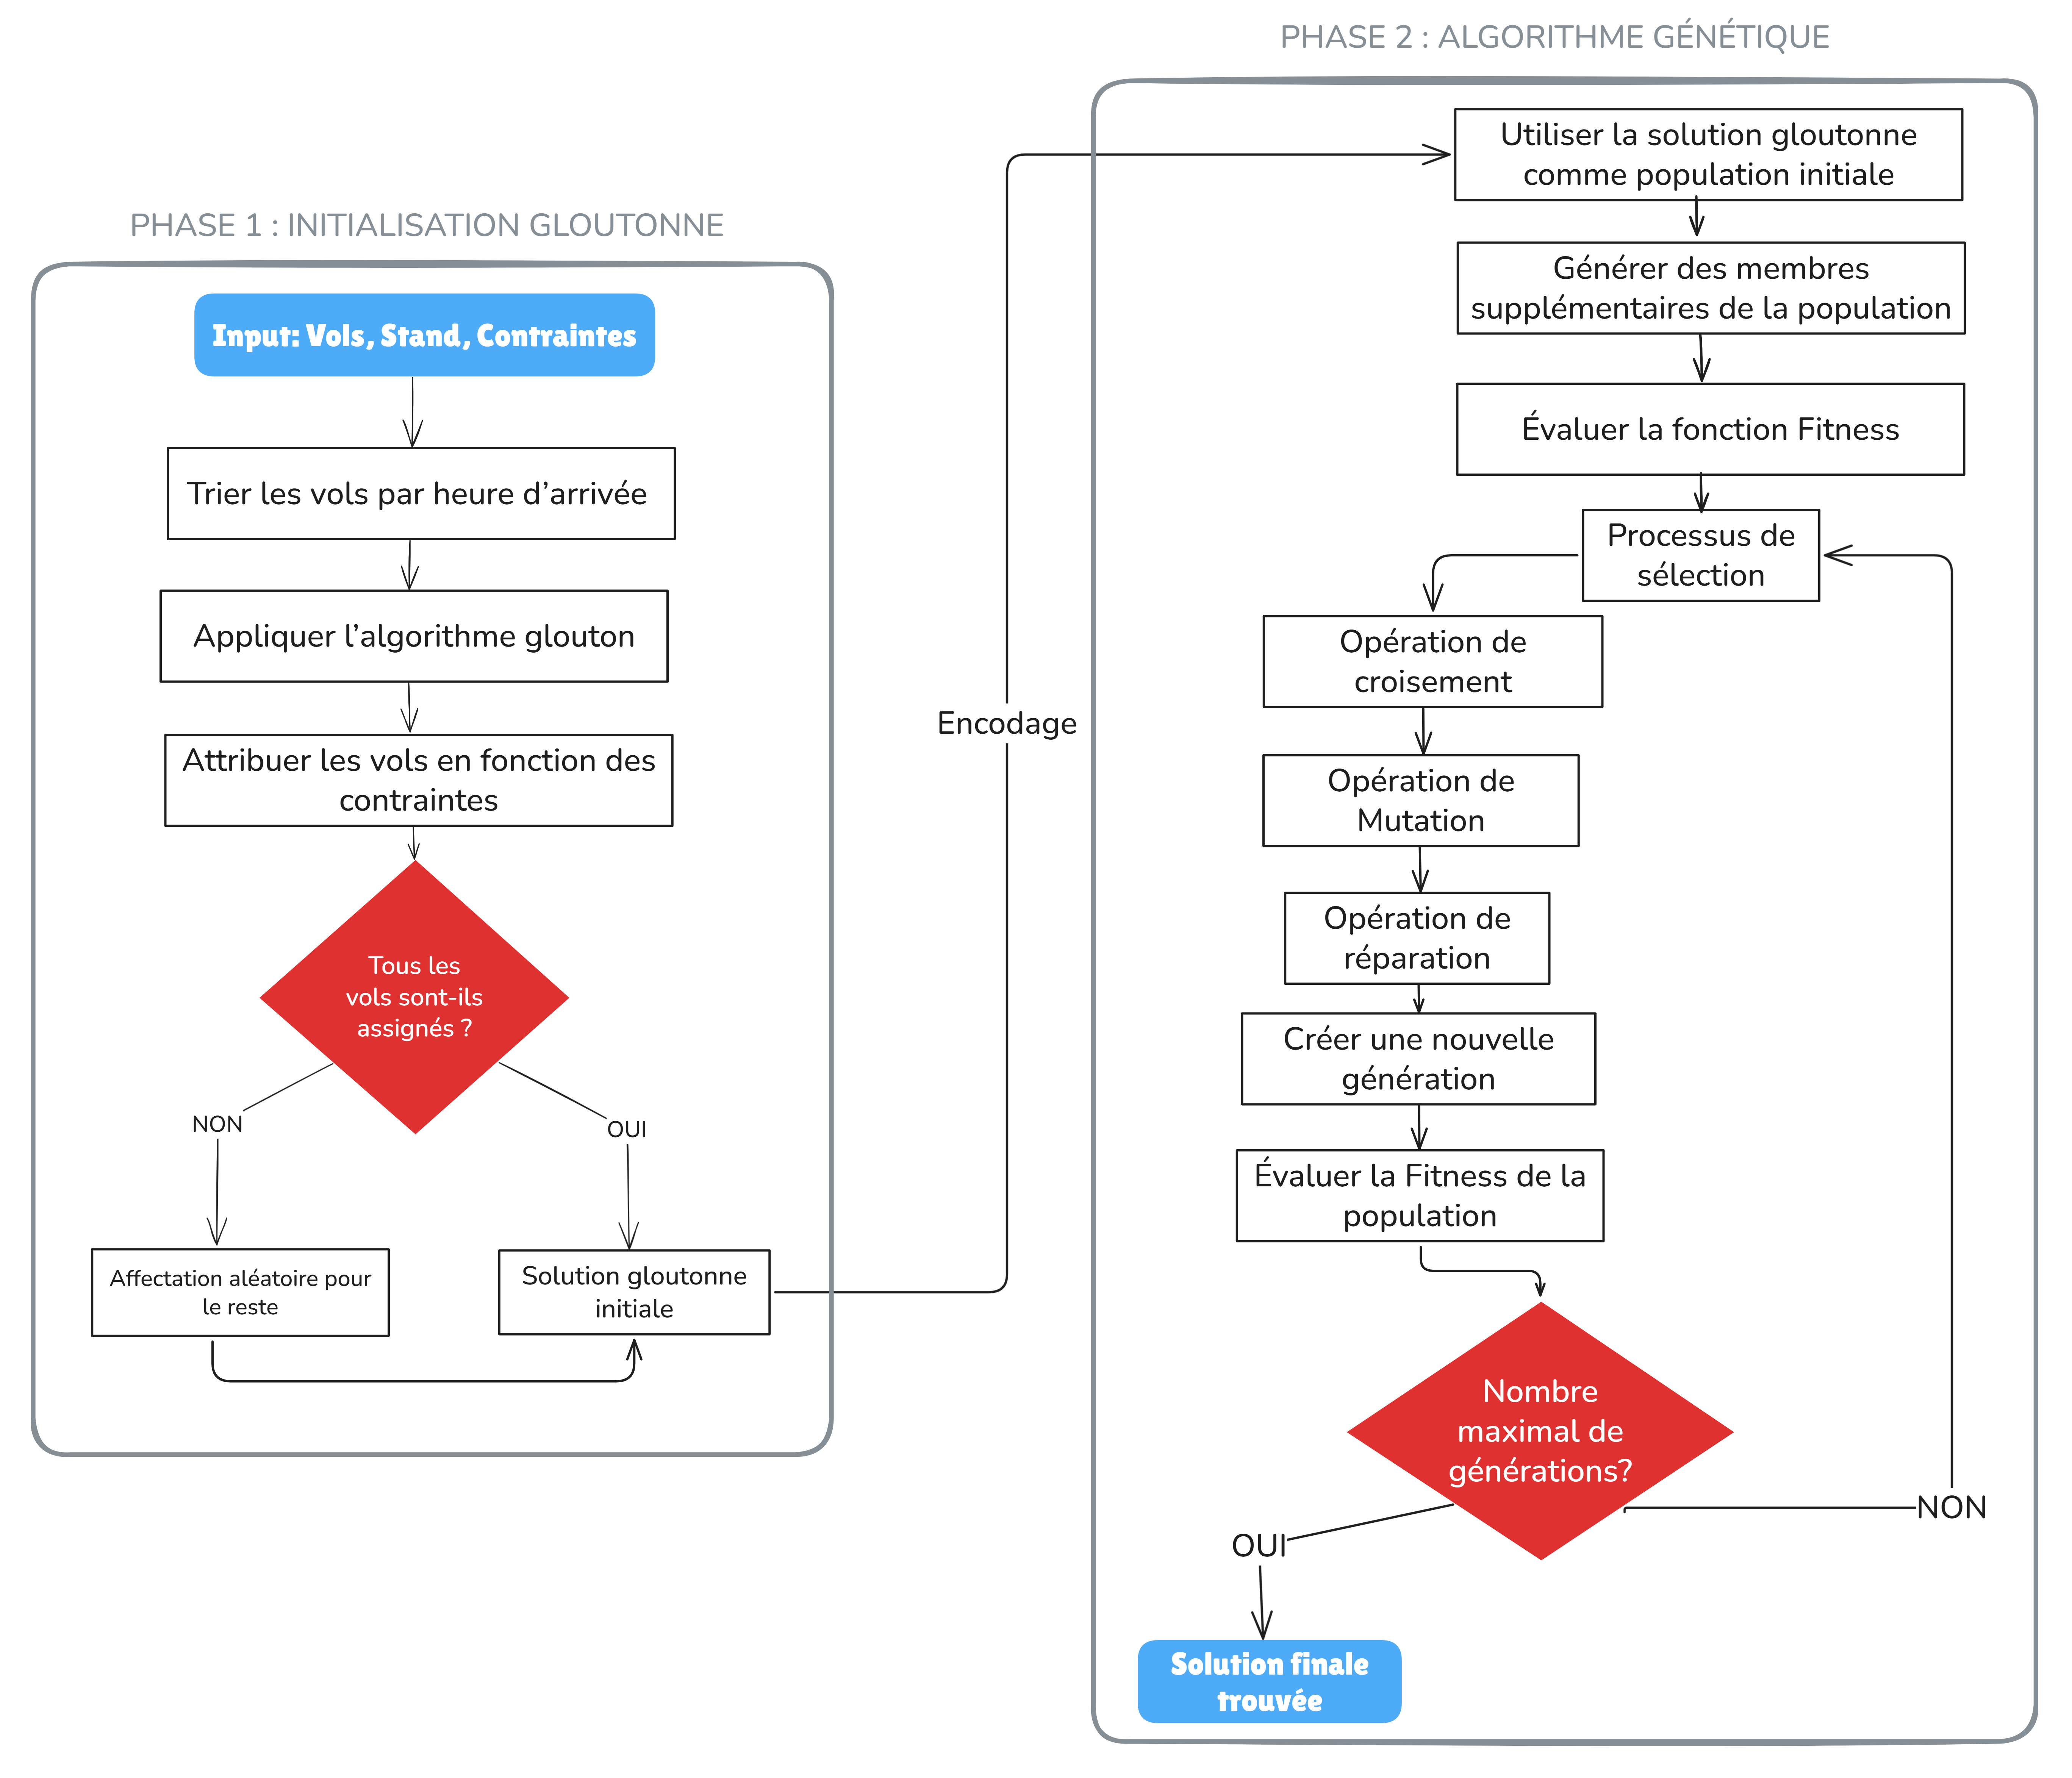
\includegraphics[width=0.9\linewidth]{assets/algo/GA_Algorithm.jpg}
	\caption{Organigramme de l'algorithme génétique}
	\label{fig:GGA}
\end{figure}
		\vspace{-0.7em}     
 Comme illustré dans la Figure~\ref{fig:GGA}, l’approche suit une structure en deux phases : la première utilise un algorithme glouton pour produire rapidement des solutions réalisables proches de l’optimal ; la seconde exploite ces solutions élites pour initialiser l’algorithme génétique, accélérant ainsi la convergence tout en améliorant la qualité des solutions.
 \vspace{-0.7em}
\subsubsection*{Approche d’hybridation}
\label{subsubsec:hybridization}

L’algorithme GGA associe la rapidité des heuristiques gloutonnes à la puissance d’optimisation des algorithmes génétiques.Cette hybridation crée un effet complémentaire dans lequel la composante gloutonne fournit des solutions initiales de qualité, et la composante évolutionnaire explore l’espace des solutions pour obtenir de meilleures affectations.

L’hybridation s’effectue en deux phases : d’abord, un algorithme glouton génère des solutions faisables en triant les vols et en appliquant des règles d’affectation basées sur les contraintes ; ensuite, ces solutions sont utilisées comme individus élites dans la population initiale de l’algorithme génétique, fournissant une base solide pour l’optimisation.
\vspace{-0.5em}
\paragraph{Initialisation par algorithme glouton}
La phase d’initialisation s’appuie sur des heuristiques gloutonnes pour générer des solutions de départ de qualité. Les vols sont triés par heure d’arrivée, et les stands sont affectés en tenant compte de la disponibilité et des contraintes de compatibilité. Cette approche permet à une grande partie de la population initiale de contenir des solutions valides et proches de l’optimum plutôt que des solutions aléatoires.

À l’issue de la première phase, la solution obtenue via l’algorithme glouton est encodée dans un format compatible avec celui attendu par l’algorithme génétique. Le mécanisme d’encodage, qui assure une transition fluide entre la représentation heuristique et celle en chromosomes, est détaillé dans la section~\ref{sssec:chromosome_encoding}.
\vspace{-0.7em}
\subsubsection{Encodage des Chromosomes}
\label{sssec:chromosome_encoding}

La représentation des chromosomes utilise un schéma d'encodage entier direct qui permet de mapper efficacement les vols aux stands.

\vspace{-0.7em}
\paragraph{Structure d’encodage}
Chaque chromosome est représenté par un vecteur d'entiers :

\begin{figure}[H]
	\centering
	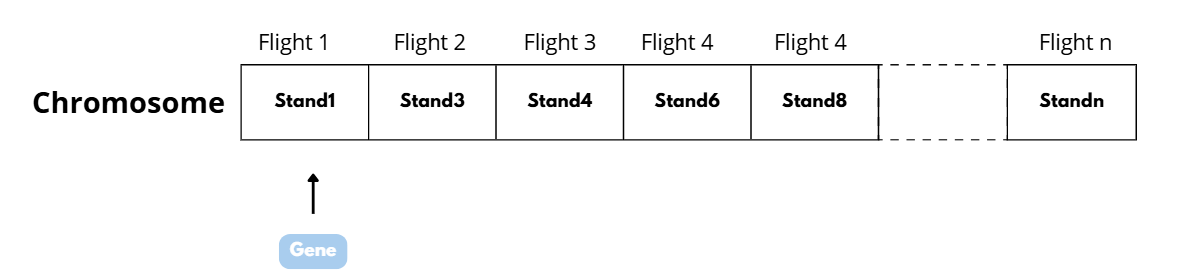
\includegraphics[width=0.9\linewidth]{assets/algo/Encodage.png}
	\caption{Structure de l’encodage}
	\label{fig:enter-label}
\end{figure}

Où :
\begin{itemize}
	\item $n$ = nombre total de vols,
	\item $Stand_i$ = indice du stand affecté au vol $i$ (gène $i$),
	\item La position $i$ correspond au vol $i$,
	\item Les valeurs des gènes vont de $0$ à $|Stands|-1$, selon le mapping (ex : B01 $\rightarrow$ 1, J01 $\rightarrow$ 2).
\end{itemize}

\paragraph{Représentation des gènes}
Chaque gène représente une affectation vol-stand :
\begin{itemize}
	\item \textbf{Indice du gène} : Position dans le chromosome (identifiant du vol),
	\item \textbf{Valeur du gène} : Entier représentant l’indice du stand dans la base,
	\item \textbf{Correspondance} : Association directe entre la valeur du gène et le stand.
\end{itemize}

\paragraph{Exemple d'encodage}
Pour les vols $F = [F_1, F_2, F_3, F_4]$ et les stands $S = [B01, C01, B02, E01, J01]$ :

\text{Chromosome}
\begin{figure}[H]
	\centering
	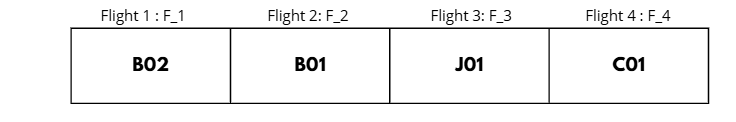
\includegraphics[width=0.7\linewidth]{assets/algo/Chr.png}
	\caption{Exemple d'encodage}
	\label{fig:enter-label}
\end{figure}
\vspace{-2em}
\begin{align}
	\text{Affectation} &= \{F_1 \rightarrow B02, F_2 \rightarrow B01, F_3 \rightarrow J01, F_4 \rightarrow C01\}
\end{align}

Cet encodage permet une efficacité computationnelle via l’indexation directe et prend naturellement en charge les opérations génétiques.

\paragraph{Processus de l’algorithme génétique}
Après l’initialisation, l’algorithme exécute les opérations génétiques standard jusqu’à satisfaction du critère d’arrêt.

\textbf{Critère d’arrêt :} l’algorithme s’arrête lorsque le nombre maximal de générations est atteint.

\paragraph{Sélection}
Les parents sont sélectionnés à l’aide d’une sélection par tournoi avec une probabilité définie, favorisant les individus avec une meilleure aptitude.

\paragraph{Croisement}
Un croisement en un point est appliqué avec une probabilité donnée. Un point de croisement aléatoire divise les chromosomes parents, permettant aux enfants d’hériter de matériel génétique des deux parents. Cela favorise la combinaison de schémas d’affectation efficaces.

\paragraph{Mutation}
La mutation s’applique avec une certaine probabilité, où un gène aléatoire est remplacé par une affectation de stand compatible. Cette opération introduit de la diversité et réduit les risques de convergence prématurée.

\paragraph{Mécanisme de réparation}
Après le croisement et la mutation, une procédure de réparation est lancée pour garantir que chaque individu respecte les contraintes du problème. Les affectations invalides causées par des conflits temporels, des incompatibilités ou des incohérences de zones sont identifiées et corrigées en réaffectant les vols vers le stand compatible le plus proche. Cette étape est essentielle pour assurer la validité des solutions tout au long de l’évolution.

\subsubsection*{Pseudocode de l’Algorithme GGA Hybride}

Le pseudocode suivant résume l’implémentation de l’algorithme génétique-glouton hybride, tel que présenté précédemment.

\begin{algorithm}[H]
	\caption{Algorithme Hybride Glouton-Génétique}
	\label{alg:gga_main}
	\begin{algorithmic}[1]
		\Require Vols $F$, Stands $S$, Contraintes $C$
		\Ensure Meilleure solution et score de fitness associé
		
		\Comment{Phase 1 : Initialisation gloutonne}
		\State Trier les vols par heure d’arrivée
		\State Générer une solution gloutonne à l’aide des règles d’affectation sous contraintes
		\State Créer la population initiale composée de variantes gloutonnes et de solutions aléatoires
		
		\Comment{Phase 2 : Évolution génétique}
		\State Initialiser la population avec les solutions gloutonnes
		\State Évaluer le score de fitness de la population initiale
		
		\While{not TerminationCriterion()}
		\Comment{Sélection}
		\State Sélectionner les parents selon la méthode de tournoi
		
		\Comment{Croisement}
		\State Générer les descendants par croisement à un point
		
		\Comment{Mutation}
		\State Appliquer une mutation pour introduire de la diversité
		
		\Comment{Réparation}
		\State Réparer les solutions non réalisables afin de respecter les contraintes
		
		\Comment{Remplacement}
		\State Remplacer la population par la nouvelle génération (avec préservation de l’élitisme)
		\State Évaluer le fitness de la nouvelle population
		\State Mettre à jour la meilleure solution si amélioration
		\EndWhile
		
		\Return Meilleure solution et valeur de fitness correspondante
	\end{algorithmic}
\end{algorithm}

%--------------------------------------------------

\section{Description des Hyperparamètres de l’Algorithme Génétique}
Cette section présente les principaux hyperparamètres utilisés dans notre approche hybride.

L’hybridation du glouton avec l’algorithme génétique utilise les hyperparamètres standards suivants :

\paragraph{Probabilité de mutation} Contrôle la probabilité d’introduire des modifications aléatoires dans une solution pour maintenir la diversité génétique et éviter la convergence prématurée vers des optima locaux.

\paragraph{Probabilité de croisement} Détermine la fréquence à laquelle le croisement entre deux parents est réalisé, équilibrant l’exploration de nouveaux espaces de solutions et l’exploitation des bonnes solutions existantes.

\paragraph{Taille de la population} Spécifie le nombre d’individus (solutions) maintenus à chaque génération. Une population plus grande améliore la diversité, mais augmente le coût de calcul.

\paragraph{Nombre de générations} Définit le nombre d’itérations de l’algorithme. Plus il y en a, plus l’exploration est profonde, mais cela allonge également le temps de traitement.

\section{Conclusion}
Ce chapitre a présenté la modélisation mathématique du problème d'affectation des vols aux stands, en s'appuyant sur une revue des approches existantes et leurs limites. Une formulation multi-objectifs a été proposée pour équilibrer l'utilisation des ressources et améliorer l'expérience passager. Nous avons également détaillé les paramètres, contraintes, et hyperparamètres associés à l’algorithme hybride glouton-génétique, en justifiant les choix méthodologiques adoptés.

Le prochain chapitre portera sur l’implémentation concrète du modèle proposé, les métriques d’évaluation, ainsi que l’analyse des résultats obtenus comparés aux affectations réelles.